\section{Introduction}
\subsection{What is HackerNews}
HackerNews is a social news site: it aggregates news by allowing users to submit stories. Interesting submissions can be upvoted by other users and all submissions are ranked by popularity.

The content on Hacker News is mostly related to science, in particular computer science. The guidelines for what content can be posted are very broad: ``\textit{anything that gratifies one's intellectual curiosity}''. This is in line with the type of companies the company behind Hacker News, YCombinator, invests in

\subsection{Research question}

\section{Dataset}
As explained in the previous section, our analysis is on the set of all stories posted on Hacker News. 

Let us first consider what we mean when we refer to a story. To do so, we have to separate between the various types of content on Hacker News, which can be catagorized in these four groups:
\begin{itemize}
\item Story: the majority of submissions are stories. A story can be either a link to another webpage or a short text by the submittor.
\item Job: companies sponsored by YCombinator (the seed investor behind Hacker News) can post job offers on Hacker News. The percentage of Jobs is very small: well under 1 of the total volume.
\item Poll: users can submit multiple choice questions for other users to answer.
\item Comment: the three types mentioned above can receive comments by other users.
\end{itemize}

Since this research focuses only on the stories, we have left out the other three types. The dataset used in our research contains all stories between February 19th 2007 (the date Hacker News was launched\footnote{\url{https://news.ycombinator.com/hackernews.html}}) and June 10th 2015 (the day we ran our crawler). This is a time span of 3033 days, during which a total of over 1.5 million stories were submitted.

To crawl all stories, we used the official Hacker News API\footnote{\url{https://hn.algolia.com/api}}. This API returns some basic data about the story, such as the submitter, title, points (upvotes), a (possibly empty) story text and a (possibly empty) url. Stories generally have either a story text or a url, most only have a url.

For the stories with a non-empty story text field, fetching it from the API is enough. For other stories, we also fetched the content the URL links to. An important remark here is that some urls (especially the old ones) have become invalid over the course of time.

\textit{Something about the article extractor GoOse}

We split the result in files with 1 day of articles per file. This dataset is about 4.4 GB in size.

\subsection{Simple statistics}
We have now established some semantics of the data gathered for our research. Before diving into the data analysis, we will first quantify the data by providing the reader with some statistics.

\subsubsection{Overall activity}

\begin{center}
    \begin{tabular}{|p{3cm}|p{3cm}|}
        \hline
        \multicolumn{2}{|c|}{Statistics} \\
        \hline
         Stories & 1544261 \\ 
         Submitters & 165126 \\ 
         Upvotes & 16668848 \\ 
         Comments & 7383865 \\
         \hline
    \end{tabular}
\end{center}

An interesting remark, is that January 6th 2014 did not have any submissions. The reason for this was a long downtime of the Hacker News website
\footnote{\url{https://twitter.com/hackernewsonion/status/420068968464789505} - Hacker News is DOWN, but your chances of getting into YC if you know how to scale a plain text website are UP.}.

\subsubsection{Top users}
In figure~\ref{fig:top10ByStories}, we show the statistics for some of the most active submitters. These statistics illustrate that Hacker News has a very active group of users. Together, this top 10 submitted 45,190 stories, which equals an average of 1.5 stories per user per day over the last 7 years.
\begin{figure}[ht!]
\caption{Top 10 submitters by submitted stories}
\label{fig:top10ByStories}
\centering
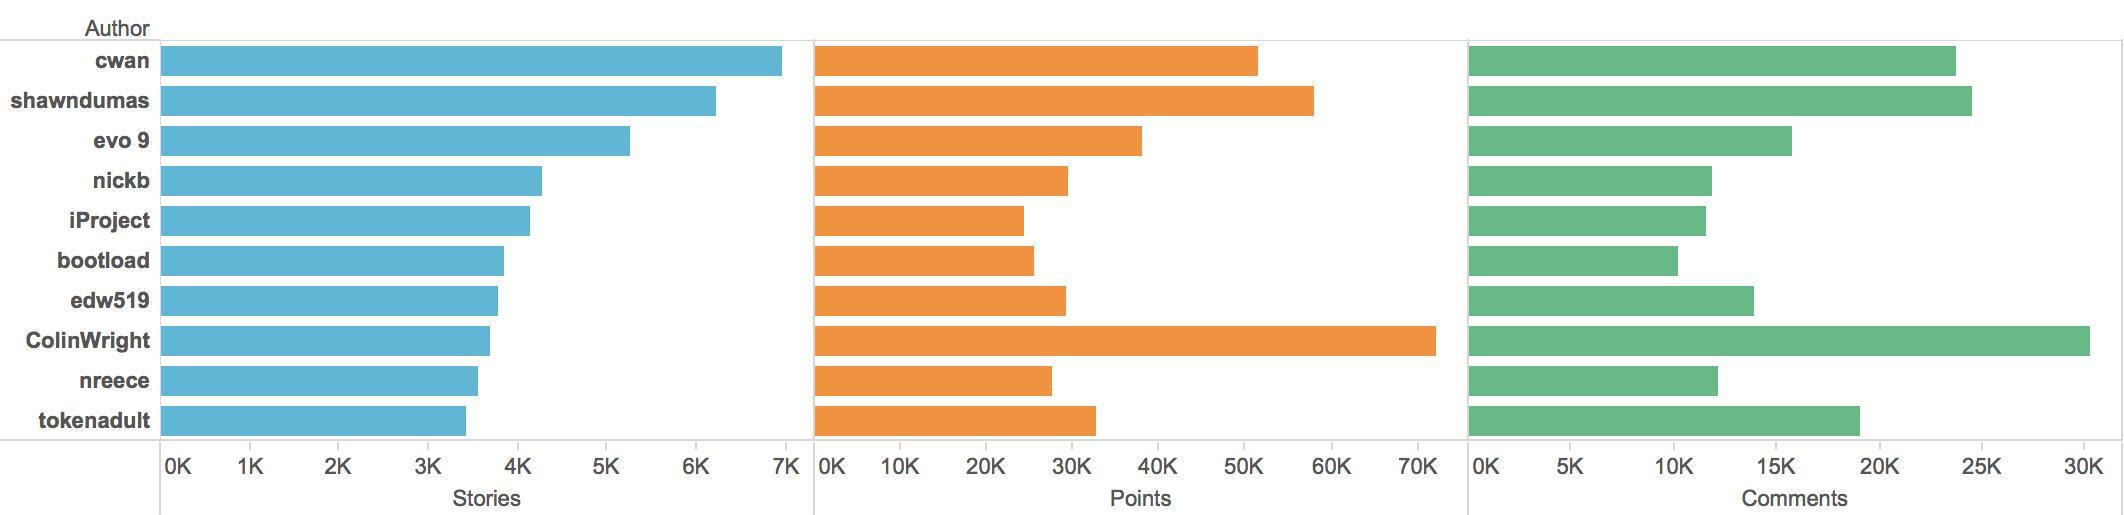
\includegraphics[width=12cm]{top10ByStories}
\end{figure}

If we take the top 10 not by the number of stories a user has submitted but by the number of comments his or her stories have received, we get the rankings in figure~\ref{fig:top10ByStories}.

\begin{figure}[ht!]
\caption{Top 10 submitters by received comments}
\label{fig:top10ByComments}
\centering
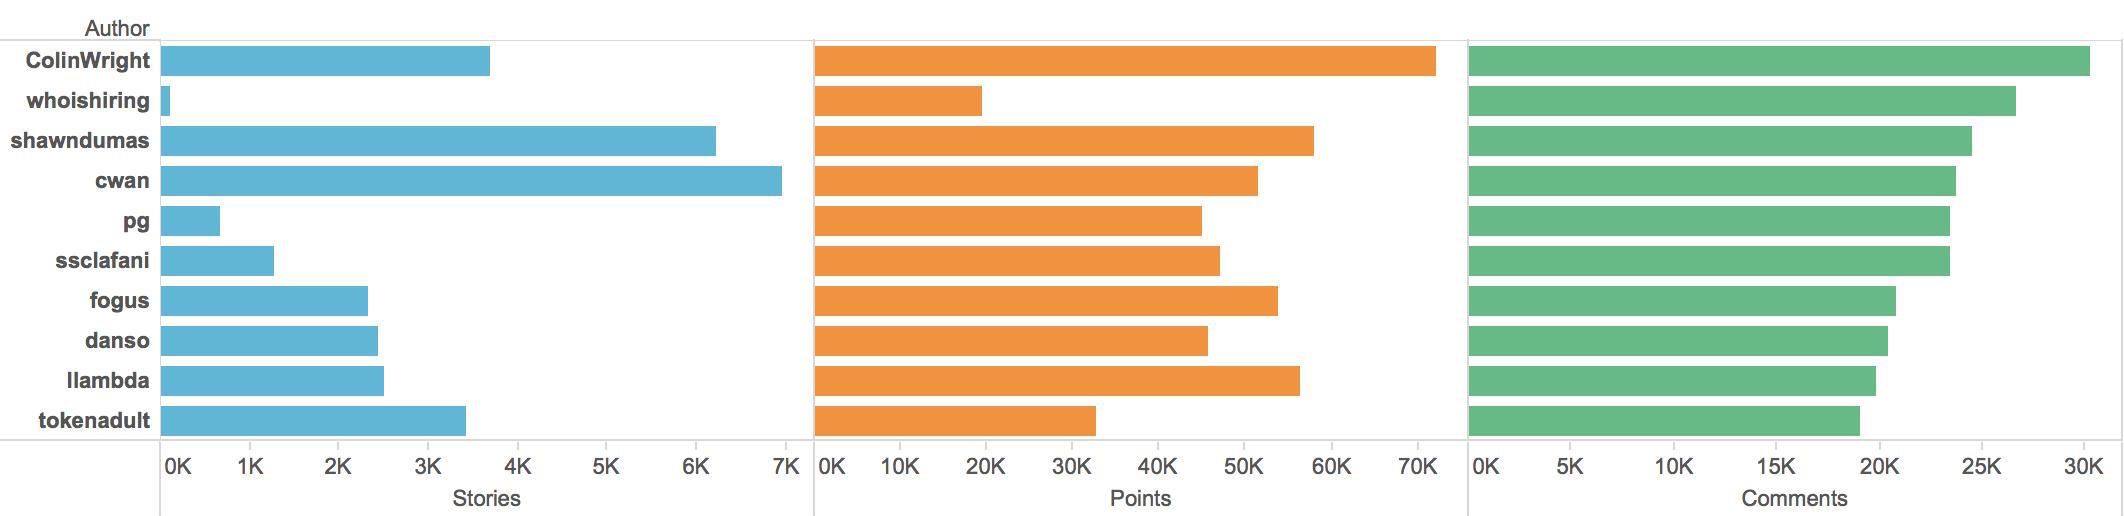
\includegraphics[width=12cm]{top10ByComments}
\end{figure}

The interesting second place in this top 10 is user ``\_whoishiring``. This user has almost no posts (a mere 114) but a massive 26,649 comments. Experienced Hacker News readers may have already expected this, for this user starts a monthly thread where companies can post job offers and others can respond to these. As such, the user only posts one story per month but its stories are discussed very actively.

\subsubsection{Top domains}
\begin{center}
    \begin{tabular}{|p{4.5cm}|p{=5cm}|p{5cm}|}
        \hline
        \multicolumn{3}{|c|}{Most popular domains} \\
        \hline
        By Stories & By Points & By Comments \\
        \hline
       techcrunch.com (27.711) 	& github.com (400.373)		       & techcrunch.com (172.854) \\
		github.com (26.596) 			& techcrunch.com (365.207) 	   & nytimes.com (153.471) \\
		youtube.com (21.977) 		& nytimes.com (287.234)		   & github.com (127.812) \\
		nytimes.com (18.125) 		& arstechnica.com (176.633)	   & arstechnica.com (80.666) \\
		medium.com (14.172) 		& wired.com (161.698)		  	   & wired.com (75.406) \\
		arstechnica.com (12.657) 	& medium.com (132.468)		   & washingtonpost.com (56.257) \\
		wired.com (10.867) 			& bbc.co.uk (98.031)		  		   & medium.com (53.924) \\
		bbc.co.uk (8.118) 				& washingtonpost.com (97.537) & bbc.co.uk (51.828) \\
		en.wikipedia.org (7.058) 		& youtube.com (96.339)		  	   & theatlantic.com (41.530) \\
		businessinsider.com (6.877) & theatlantic.com (77.628)	   & online.wsj.com (36.729) \\
         \hline
    \end{tabular}
\end{center}

\section{Analysis}
Say that we did unsupervised LDA.

\subsection{Latent Dirichlet Allocation}
Some explanation what the F*** this is

\subsection{Implementation}

\section{Results}
$1+1=10$

\section{Conclusion}
We`re awesome!